\documentclass{article}
\usepackage{graphicx,fancyhdr,amsmath,amssymb,amsthm,subfig,url,hyperref}
\usepackage[margin=1in]{geometry}
\usepackage{xltxtra}
\usepackage{xgreek}
\usepackage{amsfonts}
\usepackage{listings}
\usepackage{amssymb}
\usepackage{amsmath}
\usepackage{pdfpages}
\setmainfont[Mapping=tex-text]{Times New Roman}
%----------------------- Macros and Definitions --------------------------

%% FILL THIS OUT
\newcommand{\studentname}{Νικόλαος Ζαρίφης}
\newcommand{\suid}{03112178}
\newcommand{\exerciseset}{ SET 3}
%% END



\renewcommand{\theenumi}{\bf \Alph{enumi}}

%\theoremstyle{plain}
%\newtheorem{theorem}{Theorem}
%\newtheorem{lemma}[theorem]{Lemma}

\fancypagestyle{plain}{}
\pagestyle{fancy}
\fancyhf{}
\fancyhead[RO,LE]{\bfseries\large NTUA}
\fancyhead[LO,RE]{\bfseries\large Στοχαστικές Ανελίξεις}
\fancyfoot[LO,RE]{\bfseries\large \studentname: nick.zarifis@hotmail.com}
\fancyfoot[RO,LE]{\bfseries\thepage}
\renewcommand{\headrulewidth}{1pt}
\renewcommand{\footrulewidth}{1pt}

\graphicspath{{figures/}}

%-------------------------------- Title ----------------------------------

\title{Στοχαστικές Ανελίξεις\\ \exerciseset}
\author{\studentname \qquad  ID: \suid}

%--------------------------------- Text ----------------------------------

\begin{document}
\maketitle
\section*{Άσκησή 1}
\begin{itemize}
	\item 1
		$\sum_k \frac{x^k}{2^k} = \frac{2}{2-x}$ $x<2$ .
		Άρα μπορούμε να παραγωγίσουμε κι να πολλαπλασιασούμε με χ/2 . 
Θ έτωντας χ=1, $lhs = 1/(2-1)^2=1$. Πολύ κονα με το πρόγραμμα, 1.003 που έβγαλε.
\item 2 
	Αλλάζοντας τον κώδικα  
\lstinputlisting[language=Python,firstline=16,lastline=27]{ergodic.py}
Variance is  0.571428571429 .
\item 3
\item 4
\lstinputlisting[language=Python,firstline=9,lastline=10]{erg.py}
Γιατί ξέρουμε ότι η $\sum_k \frac{f(X_k)}{N} \rightarrow \sum_k f(k)\pi(k) $με πιθανότητα 1.
Το αποτέλεσμα που μας έβγαλε είναι: 0.468087834089.

\end{itemize}

\section*{Άσκησή 2}
\begin{itemize}
	\item 1
		Βλέπουμε ότι παράγει το ακόλουθο: 
	\\	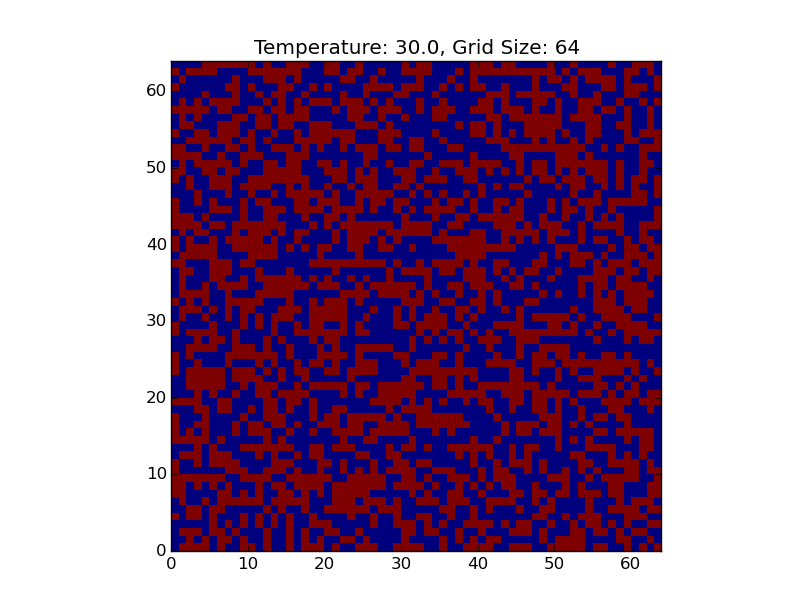
\includegraphics[heigh=100pt,width=100pt]{fig1}
       \item 2
	       βάζοντας όπου random την τιμη 1 , έχουμε το ακολουθο αποτέλεσμα:
	\\	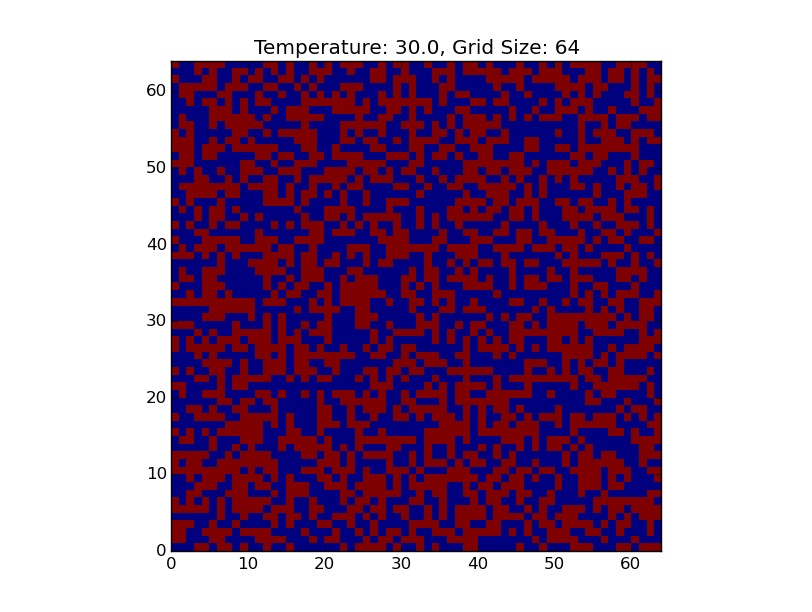
\includegraphics[heigh=100pt,width=100pt]{fig2}
		Όπως βλέπουμε, δεν υπάρχει καμοία ποιοτηκή διαφόρα στο αποτέλεσμα
	\item 3
		Αλλάζοντας τους βαθμούς στους 10 δεν παρατηρούμε τίποτα το ίδιαιτερο
		αλλά όσο μειώνουμε τους βαθμούς μένουν πολυ λίγα μπλε ή κόκκινα γενικά γίνεται μια ομογενοποιήση ενω ρυχνοντας κι άλλο την θερμοκρασία γίνονται όλα μπλε ή κόκκινα αυτό συμβαίνει γιατί όσο τίνει στο 0 όλα τα σωματίδια αποκταε ή 1 ή -1 spin απο θεωρία.
 \item 4
	 Στην μέθοδο αυτή το spin αλλάζει αν το DH ειναι αρνητικο με πιθανοτητα εα
	 το οποίο εδώ γίνεται σίγουρα γιατί θα είναι μεγαλύτερο του 1. Αν ειναι θετικό τότε το αλλάζουμε με πιθανότητα $e^{-b\Delta H}$. Εδώ έχουμε προσσεγυσει το b με 1/Τ (κανωνικα ειναι 1/κΤ). 

 \item 5
	Όπως βλέπουμε όσο μεγαλόνουμε τα βηματα τόσο ποιο μονόχρωμο γίνεται γιατί τα σωματιδια παιρνοθν την τιμη spin του γειτονα τους .
	
		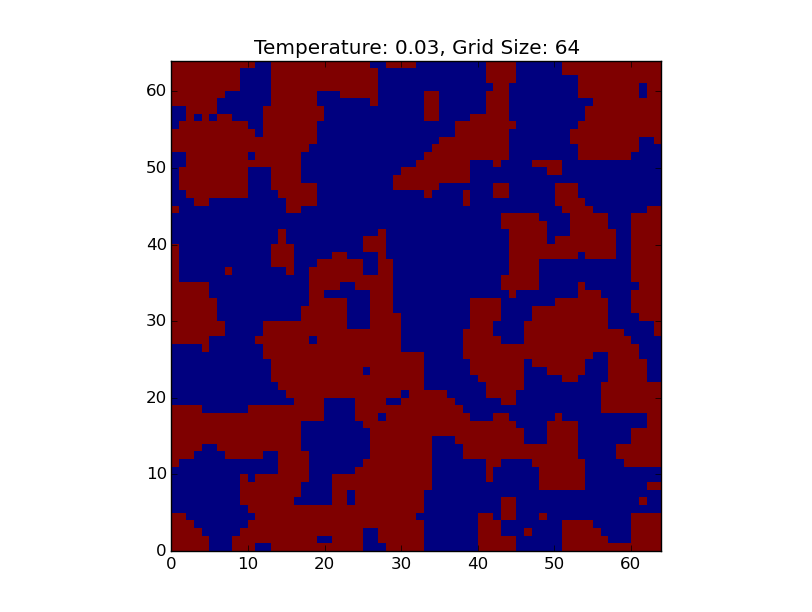
\includegraphics[heigh=100pt,width=100pt]{fig3} \\
		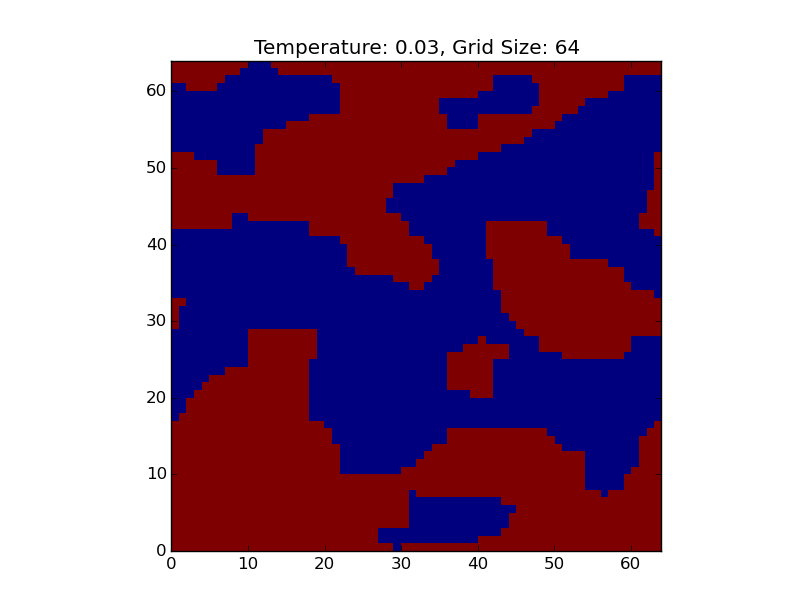
\includegraphics[heigh=100pt,width=100pt]{fig4} \\
		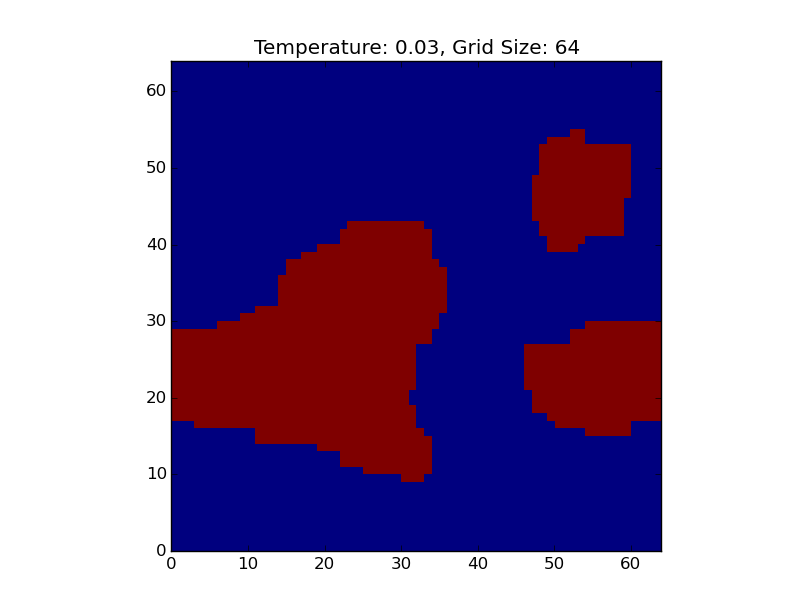
\includegraphics[heigh=100pt,width=100pt]{fig5} \\
		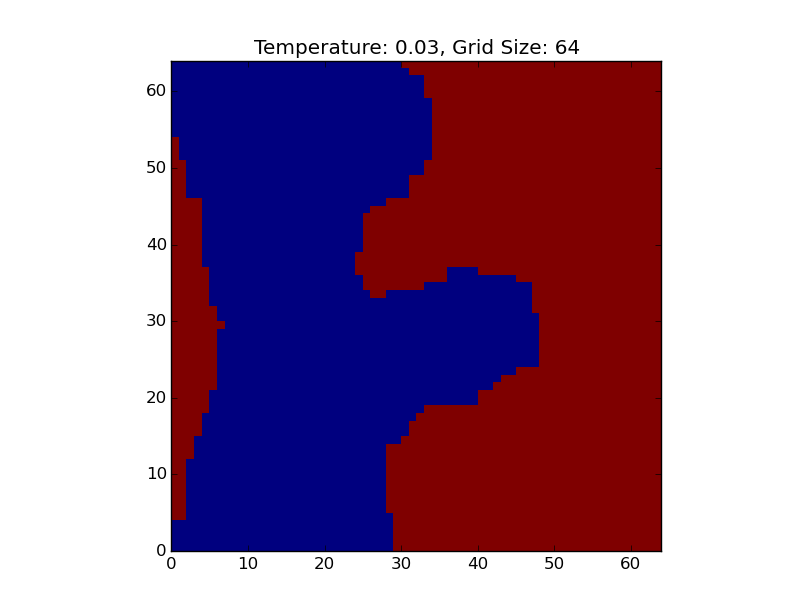
\includegraphics[heigh=100pt,width=100pt]{fig6}
\end{itemize}
\section*{Άσκησή 3}
\begin{itemize}
	\item 1
		Τρέχοντας τον κώδικα για της τιμες 1,2,3 βλέπουμε ότι σε όλες της περιπτώσεις έφτανε στο όλικο ελάχιστο, κι επίσεις για πιο μικρή τιμή παλόταν περισότερο σε χαμήλες θερμοκρασίες, μέχρι να σταθεροποιηθεί.
	\item 2
		Βλέπουμε οτι για τις τιμες 1,3 είχει 100\% επιτυχεία ενώ για 2 είχε 98,8\% .
	\item 3
		Αλλάζοντας το delta βλέπουμε ότι για 3 έχει 6.5\% για 2 έχει 45.1\% ενώ για 1 πάλι 100.Αυτό συμβαίνει γιατί για χαμήλο δελτα κάνει πιο αργές μεταβολές κι στην ουσία παραμένει στο πιο κοντίνο τοπικό ελάχιστο είναι στην αρχή, γιατί αυτό το τραβάει στην ουσία.Εξαρτάται δηλαδή απο την αρχική του θέση.
\item 4 
	Βάζοντας τον ακόλουθο κώδικα:
\lstinputlisting[language=Python,firstline=5,lastline=17]{sim2.py}
έχομουμε ως αποτέλεσμα: 
Cooling Factor:  0.5
Success Rate:  100.0\%
\\
		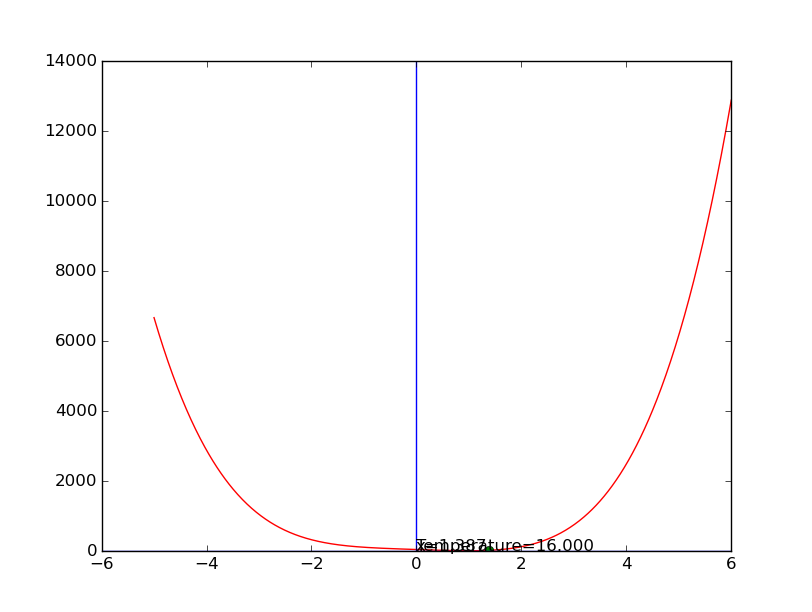
\includegraphics[heigh=100pt,width=100pt]{ex31} \\
\end{itemize}
\section*{Άσκησή 4}
\begin{itemize}
	\item 1
		Στο δεύτερο διάγραμμα , βλέπουμε ότι κατα την πάροδο του χρόνου(όσο ψυχαίνεται ) μικραίνει η απόσταση όπως ακρίβως γίνεται κι με το έλαχιστο συνάρτησεις.

		\includegraphics[heigh=300pt,width=300pt]{ex411png} \\
	\item 2
		Βλέποντας τον κώδικα βρίσκουμε οτι:\\

\lstinputlisting[language=Python,firstline=160,lastline=163]{simulatedannealingtsp.py}
\\
Βλέπουμε ότι στην αρχή υπόλογιζει την διαφόρα κι με τον ίδιο τρόπο όπως στην άσκηση 2, υπόλογιζει την πιθανότητα να αλλάξει κι να μετακινηθει.
 \item 3
Βλέπουμε το ακόλουθο αποτέλεσμα:\\
		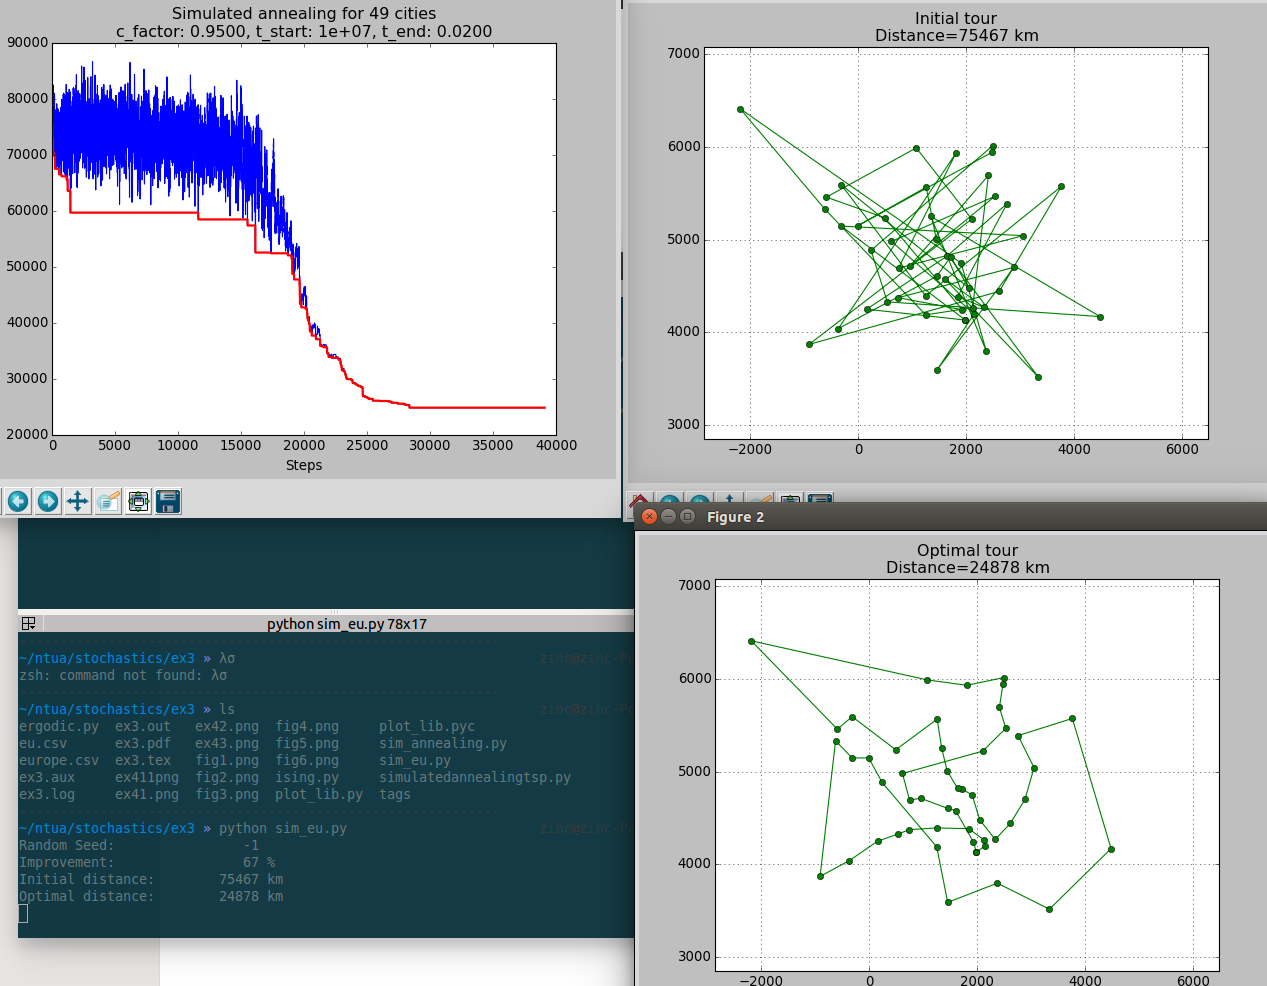
\includegraphics[heigh=300pt,width=300pt]{ex422} \\
\item 4
	Αν υποθέσουμε ότι ο γράφος μας είναι πλήρης , έχουμε συνολικά 35! μονοπάτια δηλάδη όλες οι πιθανές αναμεταθέσεις αυτός ο αριθμός είναι της τάξης $10^{40}$ , δηλάδη θα χρειαζόταν $3.23*10^{29}$ χρόνια αριθμός αρκετά μεγαλός. Βέβαια μπορούμε να χρησιμοποιήσουμε ξακήτερες προσσεγγισεις ώστε να ρίξουμε αρκετά τον χρόνο όπως DP.
\end{itemize}
\end{document}
